\documentclass{beamer}
%\documentclass[handout]{beamer}
\usepackage{etex}
\usepackage[utf8]{inputenc}
\usepackage[T1]{fontenc}
%\usepackage[english]{babel}
\usepackage{tree-dvips}
\usepackage{color}
\usepackage{colortbl}
\usepackage{amsmath}
\usepackage{amsfonts}
\usepackage{amssymb}
\usepackage{mathabx}
\usepackage{textcomp}
\usepackage{natbib}
\usepackage{tocvsec2}
\usepackage{xyling}
\usepackage{multirow}
\usepackage{nicefrac}
\usepackage{multicol}
\usepackage{url}
\usepackage{tree-dvips}
\usepackage{gb4e-}

\title[Token-level noise and non-destructive normalization]{\Large Token-level noise in large web corpora\\
and non-destructive normalization\\
for linguistic applications}
\author[Felix Bildhauer, Roland Schäfer]{\Large Felix Bildhauer and Roland Schäfer}
\institute{SFB 632/A2, German Grammar and Linguistics (FU Berlin)}
\date{CANS, Lancaster, July 22, 2013}

\usetheme{FUBerlin}
%\definecolor{beamer@fuorange}{rgb}{.9,0.5,0.1}
\definecolor{beamer@fuorange}{rgb}{.8,.3,0}
\definecolor{Gray}{gray}{0.5}
\definecolor{Black}{gray}{0}
\setbeamercolor{alerted text}{fg=beamer@fuorange}
\titlegraphic{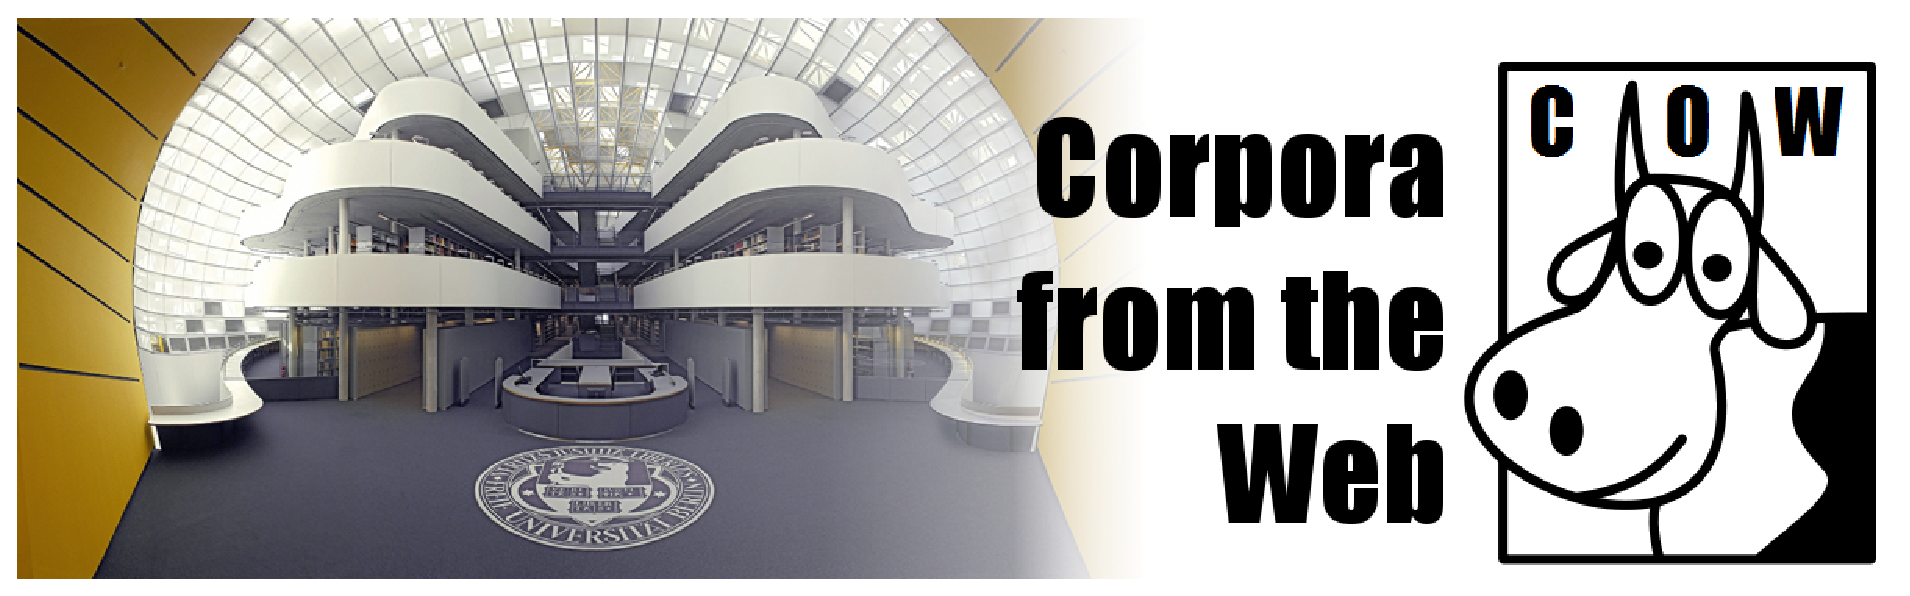
\includegraphics[height=3cm]{muhkuh}}%
\fuberlinlogon{0.8cm}
\renewcommand{\fuberlinfootstring}{\insertshortauthor{} \number\year, \insertshortinstitute}

\setcounter{tocdepth}{1}

\AtBeginSection[]
{
  \settocdepth{subsection}
  \begin{frame}
    \frametitle{We are here\dots}
%      \begin{multicols}{2}
         \footnotesize
         \tableofcontents%[currentsection, hideothersubsections]
%      \end{multicols}
   \end{frame}
  \settocdepth{subsubsection}
}

\newcommand{\xxx}{\hspaceThis{[}}

\newcommand{\Lf}{
  \setlength{\itemsep}{1pt}
  \setlength{\parskip}{0pt}
  \setlength{\parsep}{0pt}
}

\newcommand{\graw}[1]{{\color[rgb]{0.8,0.8,0.8}#1}}
\newcommand{\blaw}[1]{{\color[rgb]{0.2,0.2,0.9}#1}}
\newcommand{\grien}[1]{{\color[rgb]{0.1,0.6,0.1}#1}}
\newcommand{\myalert}[2]{{\color<#1>[rgb]{0,0.7,0}#2}}
\newcommand{\eg}{e.\,g.}
\newcommand{\Eg}{E.\,g.}
\newcommand{\ie}{i.\,e.}
\newcommand{\Ie}{I.\,e.}
\newcommand{\Dim}{\cellcolor{Gray}}
\newcommand{\Off}{\cellcolor{Black}}

\newcounter{lastpagemainpart}

\begin{document}

\fuberlintitlepage[12pt]

\begin{frame}
  \footnotesize
  \vspace{0.1cm}
  \begin{center}
    COW project:\\
    \alert{\url{http://hpsg.fu-berlin.de/cow/}}\\
    \vspace{0.3cm}

    \texttt{texrex} (current version: \texttt{texrex-hyperhyper}):\\
    \alert{\url{http://sourceforge.net/projects/texrex/}}
    \vspace{0.3cm}

    \textbf{Our brand new book on web corpora}:\\
    \alert{\url{http://sites.morganclaypool.com/wcc/}}\\
    \alert{\url{http://www.morganclaypool.com/toc/hlt/2/1}}
  \end{center}
\end{frame}

\begin{frame}
  {Overview}
%    \begin{multicols}{2}
       \footnotesize
       \tableofcontents[hideallsubsections]
%    \end{multicols}
\end{frame}

\section{Introduction: Noise in web corpora}

\begin{frame}
  {Dimensions of noisiness}
  \begin{center}
    \begin{tabular}{lrl}
      \hline
      N tokens:         & 9,108,097,177&\\
      N types:          & 63,569,767&\\
      N hapax legomena: & 39,988,127&\\
      \hline
    \end{tabular}\\

    \vspace{0.8cm}
    {\tiny Proliferation of types: type and token counts for German web corpus DECOW2012\\
      \cite{Schaefer-Bildhauer2012a,SchaeferBildhauer2013}\\
      similar results in \cite{LiuCurran2006}}
  \end{center}
\end{frame}

\begin{frame}
  {Noise in web corpora}
  \begin{center}
    
    \begin{tabular}{lrr}
      Source & \% & 95\% CI ($\pm\%$)\\
      \hline
      misspelling               & $20.0$ & $5.0$\\
      tokenization error        & $17.6$ & $4.7$\\
      non-word                  &  $7.6$ & $3.3$\\
      foreign-language material &  $6.8$ & $3.1$\\
      \hline
      rare word & $46.8$ & $6.2$ \\
      number    &  $1.2$ & $1.3$ \\
    \end{tabular}\\

    \vspace{0.3cm}
    {\tiny Classification of hapax legomena in DECOW2012;\\
    estimated proportions of different categories ($n=250$), with 95\% confidence interval (CI)\\
    \cite{SchaeferBildhauer2013}}
  \end{center}
\end{frame}

\begin{frame}
  {Classification of errors in POS tagging}
  The background of the work presented here:
  \begin{itemize}
    \item improve linguistic post-processing (considerably\\
      lower quality in web corpora, \citealp{GiesbrechtEvert2009})
    \item allow users to also retrieve misspelled words etc.
  \end{itemize}
  \begin{center}
    \scalebox{0.7}{
      \begin{tabular}{l|r}
	\hline
	Class & \% \\
	\hline
	non-standard orthography & $32.3$\\
	lexicon gaps& $19.8$  \\
	foreign language material &  $18.9$\\
	emoticons &  $13.7$\\
	named entities &  $5.4$\\
	tokenization errors &  $3.1$\\
	other &  $6.8$\\
	\hline
      \end{tabular}
    }\\

    \vspace{0.3cm}
    {\tiny sample drawn from a sub-corpus of DECOW2012 containing predominantly informal language}
  \end{center}
\end{frame}

\begin{frame}
  {Breakdown of non-standard orthography (DECOW2012)} 
  \begin{center}
    \begin{tabular}{l|r}
      \hline
      Class & \%\\
      \hline
      genre-specific spellings & $59.2$\\
      omitted whitespace & $13.4$\\
      variants        & $19.7$\\
      ordinary typos & $7.56$\\
      \hline    
    \end{tabular}
  \end{center}
\end{frame}

\section{HyDRA -- Hyphenation removal}

\begin{frame}
  {Hyphenated words in web corpora}
  \begin{itemize}
    \item sources: pasted material from word processors, etc.
    \item disadvantage: no line endings as additional hint,\\
      \cite{GrefenstetteTapanainen1994} too naïve
    \item little discussion available, e.\,g., \cite{Zamorano2011} 
  \end{itemize}
\end{frame}

\begin{frame}
  {Examples of type I: Merge}
  \begin{itemize}
    \item \alert{Seiten- streifen} $\Rightarrow$ Seitenstreifen (\textit{hard shoulder})
    \item \alert{an- wählen} $\Rightarrow$ anwählen (\textit{select\slash dial})
    \item \alert{E- missionen} $\Rightarrow$ Emissionen (\textit{emissions})
    \item \alert{Physio- kratie} $\Rightarrow$ Physiokratie (\textit{Physiocracy})
  \end{itemize}

  \vspace{0.5cm}
  {\tiny All examples are from DECOW2012 (German) or UKCOW2012 (English)}
\end{frame}

\begin{frame}
  {Examples of type II: Concatenate}
  \begin{itemize}
    \item \alert{Philipps- Lagerverkauf} $\Rightarrow$\\
      Philipps-Lagerverkauf (\textit{Philips stock sale})
    \item \alert{U- Bootalarm} $\Rightarrow$ U-Bootalarm (\textit{submarine alert})
    \item \alert{5- Alpha-Reduktase-Hemmer} $\Rightarrow$\\
      5-Alpha-Reduktase-Hemmer (\textit{5-alpha-reductase inhibitor})
    \item \alert{18- karätigem} $\Rightarrow$ 18-karätigem (\textit{18-carat})
  \end{itemize}
\end{frame}

\begin{frame}
  {Examples of type III: Leavealone}
  \begin{itemize}
    \item \alert{deutsch- u.} bald auch der englischsprachigen Blogosphäre\\
      \textit{the German- and soon also the English-speaking blogosphere}
    \item \alert{Film- und} Entertainment-Gesellschaft\\
      \textit{movie(-) and entertainment society}
    \item die \alert{Innen- gegenüber} der Außenentwicklung\\
      \textit{the domestic(-) versus the foreign development}
    \item weder ein \alert{TV- noch} ein Radiosender\\
      \textit{neither a TV(-) nor a radio station}
    \item jeder \alert{Sport- insbesondere} Volleyballbegeisterte\\
      \textit{each sports(-), especially volleyball fan}\\
  \end{itemize}
\end{frame}

\begin{frame}
  {English examples}
  \begin{itemize}
    \item It has a \alert{graph- ing} facility for scatterplots (Merge)
    \item any child whose \alert{self- esteem} needs a boost (Concatenate)
    \item I called upon my \alert{Uranus- Neptune} entity (Concatenate)
    \item horseriding, and \alert{hang- and} paragliding (Leavealone)

      \vspace{0.5cm}
    \item some \alert{cases- and} interpretation - of classic 1960s\\
      D-class movies (actually type IV: Dashify, currently ignored,\\
      i.\,e., treated as Leavealone)
  \end{itemize}
\end{frame}

\begin{frame}
  {HyDRA -- Hyphenation Detection and Repair Application}
  Common HyDRA component uses frequencies of bigram $b$\\
  (of the form \alert{A- B}) and the frequencies\\
  of its dehyphenation transformations from the corpus:\\
  \vspace{0.3cm}
  \begin{itemize}
    \item frequency of the bigram itself: $f(b)$
    \item frequency of the concatenation of the bigram: $f(C(b))$
    \item frequency of the merge of the bigram: $f(M(b))$
    \item currently \alert{not even frequencies of the two parts}
    \item currently \alert{raw frequencies}, no (smoothed) probabilities
  \end{itemize}
\end{frame}

\begin{frame}
  {Decision}
  \begin{center}
    The HyDRA API offers one function \texttt{hydra()}, which\\
	
    \vspace{1cm}
    \onslide<2->{\large \alert{returns the most frequent of\\
        $b$, $C(b)$, and $M(b)$}}\\

	\vspace{1cm}
	\onslide<3->{This was our first ``baseline'' attempt\ldots\\
	and we left it at this.}
  \end{center}
\end{frame}

\begin{frame}
  {Evaluation}
  \begin{itemize}
    \item data and frequencies from a DECOW2012 slice (1.5 bn tokens)
    \item n=684 
    \item \alert{type accuracy 63.7\%}
    \item \alert{token accuracy 99.6\%}\\
      (tokens of the types from the sample in the whole corpus)
    \item primary reason for low type accuracy:\\
      Many separated nominal compounds with ``-''\\
      are not concatenated when concatenation is unseen.
    \item example: \textit{Foto- Frau} $\Rightarrow$ \textit{Foto-Frau}
  \end{itemize}
\end{frame}

\begin{frame}
  {Solutions considered\slash chosen}
  \begin{itemize}
    \item use unigram frequencies of parts of the bigram\\
      (probably useless)
    \item \ldots or use a language-specific rule for German\\
      based on mixed capitalization of German nouns
    \item \alert{one} simple exception rule -- quite effective:\\
      \alert{If both parts have mixed capitalization, Concatenate!}
    \item \alert{Type-Accuracy 91.8\% (+28.1\%)}
    \item \alert{Token-Accuracy 99.9\% (+0.03\%)}
    \item downside: does not generalize to other languages,\\
      rules and evaluations for other languages missing
  \end{itemize}
\end{frame}

\include{spellingbee}
\section{Non-destructive normalization}

\begin{frame}
  {Reasons for non-destructive normalization}
  \begin{itemize}
    \item our goal: carefully sampled and processed web corpora\\
      for fundamental research -- theoretical linguistics,\\
      linguistic web characterization
    \item \alert{noise or distortion through processing intolerable}
    \item \alert{Leave major destructive design decisions to the user!}
  \end{itemize}
\end{frame}

\begin{frame}
  {Web data specific research}
  \begin{itemize}
    \item findings in \citeauthor{SchaeferSayatz2013} (submitted):\\
      non-standard cliticized forms of the German indefinite article\\
      are frequent in web data, totally absent elsewhere
    \item \textit{ein} $\Rightarrow$ \textit{n}, \textit{einem} $\Rightarrow$ \textit{nem}, etc.
    \item longstanding morpho-syntactic\\
      and graphemic hypotheses made testable
    \item \alert{In such cases, aggressive destructive normalization\\
      removes features from the corpus which make it unique!}
  \end{itemize}
\end{frame}


\begin{frame}
  {Non-destructive normalization in COW2013}
  Spelling correction can be represented as annotation layer.\\
  (Dehyphenation cannot, at least not efficiently.)\\

  \vspace{0.3cm}
  \begin{center}
    \scalebox{.6}{
    \begin{tabular}{llllll}
      \hline
  \textbf{Word} & \textbf{POS} & \textbf{Lemma} & {\textbf{Corr.Word}}& {\textbf{Corr.POS}}& {\textbf{Corr.Lemma}}\\[1ex]
      \hline

  \ldots  &               &               &{\ldots}   &               &               \\
  the     &DT&	the 	&{the}	&{DT}	&{the} 	\\
  players	&NNS&	player	&{players}  &{NNS}	&{player}	\\
  play	&VBP&	play	&{play}	&{VBP}	&{play}	\\
  .	&SENT&	.	&{.}	&{SENT}	&{.}	\\
  The	&DT&	the	&{The}	&{DT}	&{the}	\\
  FA	&NP&	FA	&{FA}	&{NP}	&{FA}	\\
  does	&VBZ&	do	&{does}	&{VBZ}	&{do}	\\
  \alert{abosolutley}&\alert{JJ}&\alert{$<$unknown$>$}& {\alert{absolutely}}&	{\alert{RB}}	&{\alert{absolutely}}       \\
  nothing	&NN&	nothing	&{nothing}  &{NN}	&{nothing}	\\
  to	&TO&	to	&{to}	&{TO}	&{to}	\\
  help	&VB&	help	&{help}	&{VB}	&{help}	\\
  Clubs	&NNS&	club	&{Clubs}	&{NNS}	&{club}	\\
  \ldots&                 &                &  \ldots   &  &\\               
      \hline
    \end{tabular}
    }
  \end{center}
\end{frame}


\begin{frame}
  {Summary}
  \begin{itemize}
    \item Web corpora are noisy, but the noise is valuable data,\\
      and the valuable data is noise.
    \item High-quality dehyphenation is surprisingly simple \graw{for German}\\
      and need not\slash cannot be executed non-destructively.
    \item Spelling correction is (still) as difficult as we knew it was.
    \item Huge non-destructively normalized web corpora are possible\\
      and, in fact, available (soon).
  \end{itemize}
\end{frame}

% --------------- REFS + APPENDIX

\begin{frame}[allowframebreaks]
{References}
\def\newblock{\hskip .11em plus .33em minus .07em}
\tiny
\bibliographystyle{abbrvnat} 
\bibliography{cowbib}
\end{frame}

\makeatletter
\setcounter{lastpagemainpart}{\the\c@framenumber}
\makeatother

%\appendix
%\section{Appendix}

\mode<beamer>{\setcounter{framenumber}{\thelastpagemainpart}}
\end{document}
